\documentclass{article}
\usepackage{geometry}
\geometry{a4paper,left=3.5 cm,right = 3.5 cm, top=2.5 cm, bottom=2.5 cm}
\usepackage{ctex}
\usepackage{amsmath}
\usepackage{graphicx}
\usepackage{subfigure}
\usepackage{multirow}
\usepackage{booktabs}
\usepackage{float}
\usepackage{amssymb}
\usepackage{setspace}
\usepackage[colorlinks,
            linkcolor=red,
           	anchorcolor=blue,
           	citecolor=green]{hyperref}
\usepackage{natbib}
\usepackage{listings}
\usepackage{fancyhdr}
\pagestyle{fancy}    
\rhead{\bfseries 高级计量经济学II 期末论文}  

% Sef-defined Commands lol!!!
\newcommand{\enabstractname}{Abstract}         % For Engish Abstract. What the hell?
\newenvironment{enabstract}{%
    \par\small
    \noindent\mbox{}\hfill{\bfseries \enabstractname}\hfill\mbox{}\par
    \vskip 2.5ex}{\par\vskip 2.5ex}

\author{北京大学经济学双学位 \\ 潘斌 \\ W15194142}
\title{上市公司财务报表错报的预测 \\ 基于中国资本市场2002年至2017年数据的分析}

\begin{spacing}{1.5}
\begin{document}
\kaishu
\maketitle
	%\pagebreak
	\begin{abstract}
    \par 本文基于 2002 年至 2017 年中国资本市场的数据,比较 logit 模型和决策树类模型对于上市公司财务报表错报的预测力。本文首先对原始样本使用 SMOTE 算法进行过采样,以处理原始样本中类不平衡的问题。之后,本文进行 logit 模型、CART 和随机森林的算法的预测与评估。研究结果显示: SMOTE 算法确实能够提升三个模型查准率;传统的 logit 模型预测的精准度为 67.3\%,而决策树类的模型精准度超过80\% 且具有更大的AUC 值。在使用梯度优化法对于随机森林模型调参后,模型AUC 达 0. 763。本文认为使用随机森林算法能够更好帮助利益相关者发现财务报表重大错报
    \par \textbf{关键词:} 财务报表错报 \quad 决策树 \quad 随机森林
	\end{abstract}
    \pagebreak
	\begin{enabstract}
    \par Based on the data of China's capital market from 2011 to 2017, this paper uses three statistical learning models to predict the misstatement of listed companies' financial statements. Before making the prediction, this paper first uses the SMOTE algorithm to oversample the original sample to deal with the unbalance problem in the original sample. Predict and evaluate logit models, CART, and Random Forest algorithms. The research results show that the problem of class imbalance does exist in the forecasting problem of misstatement of financial statements, and the SMOTE algorithm can indeed improve the precision of the three models; the accuracy of the traditional logit model in predicting the Chinese capital market is 67.3\%, and the model accuracy of the decision tree and random forest is more than 80\% with a larger AUC value. Afterwards, this paper uses the gradient optimization method to tune the random forest model. The AUC of random forest model after tuning is 0.763.
    \par \textbf{Keywords:} Misstatements \quad CART \quad Random Forest 
    \end{enabstract}
    \pagebreak
\section{引言}
\par 我国资本市场乱象横生,形形色色的问题一经爆出,就会使得投资者、监管者和其他利益相关方蒙受巨大的损失。每年证监会都会披露上市公司的违规信息\footnote{见证监会官网,行政处罚:http://www.csrc.gov.cn/pub/zjhpublic/}。违规中有一部分是上市公司高管为了一己私利的个人违规行为,而另一部分是上市公司为了避免退市而进行的报表操纵。无论哪一类违规都会对公司的财务报表造成扭曲,影响公司价值。然而,这些违规证监会需要经过一段时间的调查才能得出结论,因此信息公开的时间都是滞后的(之后几个月甚至数年)。因此,本文意在建立一个能通过公司财务与非财务特征,快速评估公司当年是否可能违规的预测模型。同时,本文还想探究决策树等统计学习手段是否比传统logit回归在预测问题上更具有效率。
\par 为什么有了审计师和审计报告还需要统计学习呢?被审计的上市公司需要付钱给审计师事务所。所以审计师和被审计单位是有利益相关关系的。在我国,每年出具的大部分审计报告都是标准无保留意见。然而,每年又有10\%以上的公司因为错报被证监会审查。统计学习的介入,既能帮助审计师快速评估一个公司的情况,减少审计成本;又能给其他利益相关者以参考。
\par 要建立预测模型主要有三个挑战:第一、检查违规行为是一个大海捞针的行为\cite{Perols2015Finding}。每年违规的公司相对于没有违规(没有被发现违规)的公司是比例较少的。本文所用的数据集中,违规的比例是16\%\footnote{由于证监会调查滞后性,很多公司的违规行不会只持续一年,调查的结果可能是连续数年的违规。}。数据的稀缺性\footnote{即,类不平衡的问题(imbalanced dataset)。}可能使得模型的拟合困难。第二、相对于较少的公司,有太多的变量可供选择\cite{Perols2015Finding}。这些变量可能造成过拟合。本文所采用的变量是在经过国外检验的公认的对于识别有效的变量。第三、违规行为的异质性。违规行为如虚列资产和延迟披露等,其危害程度是不尽相同的。尽管如此,大部分文章将所有的违规视作相同类型进行处理\footnote{即,设定违规与不违规为一个二分变量,不对违规程度做区分。}。这样做的好处是十分简便。本文也将沿用这种设定。
\par 本文首先对训练集采用SMOTE(Synthetic Minority Over-sampling Technique)\cite{Chawla2002SMOTE}算法进行过采样,以解决类不平衡的问题。之后, 本文整理了盈余管理、公司绩效、非财务数据等特征,并进行如下几个模型的预测:第一是logit模型;第二是决策树;第三是随机森林。在进行时,本文使用交叉验证以避免过拟合。
\par 本文发现:决策树和随机森林模型在经过调参后能够击败logit模型,具有更好的预测能力和更大的AUC值。进过调参后的随机森林模型的AUC值为0.763,比logit模型高近0.16。决策树模型的准确率为83.1\%,比logit回归高近13百分点。其次,本文给出了有决策树计算出的特征重要性排序,和连续变量的最优划分\footnote{由CART算法给出}。据此本文认为决策树和随机森林算法能够更好的帮助利益相关者尽快发现上市公司的报表问题。
\par 本文的结构安排如下:第一部分是引言;第二部分回顾相关文献;第三部分阐述了本文的研究背景和初步分析;第四部分介绍本文使用的数据和统计学习模型;第五部分报告了实证的结果并进行模型评估;第六部讨论了本研究的结论和意义。

\section{背景以及相关分析}
\par 美国从本世纪初就开始关注财务报表的欺诈侦测 (fraud detection),亦可称为财务报表错报的预测问题。在2000年,Bell和Carcello\cite{Bell2000A}整理了一个包含77个错报公司和305个非错报公司的样本,并使用logit模型进行回归。他们发现较弱的内部控制、较快的公司增长速度和不正常的利润率是上市公司可能发生报表欺诈的标志。至此之后, 一部分的文献集中于盈余管理与内部控制关系,这些文章将盈余管理当作财务报表质量的代理变量\cite{Mark1996An}\cite{DechowP1996Causes}\cite{Summers1998Fraudulently}。另一部分则集中研究什么变量能够显著的帮助审计师解释财报质量\cite{Dechow2011Predicting}\cite{Felo2007Using}\cite{Ettredge2011Is}\cite{Dechow2006The}\cite{Beneish1997Detecting}
国内的研究集中在盈余管理与重大错报风险的相关关系上,一般认为盈余管理程度高的公司具有更高的重大错报风险\cite{孙欣然2015盈余管理、分析师盈余预测与重大错报风险}。本文借鉴了上述研究所用的上市公司特征。
\par Varian\cite{Varian2014Big}认为当下的计量经济学学家应该更多借助统计学习工具去研究课题。近年来,很多的研究采用了如支持向量机(SVM)、决策树分类器和一些集成算法等统计学习工具,并取得了比传统的计量工具更好的预测准确率\cite{Whiting2012Machine}。David和Hansen等人\cite{Whiting2012Machine}利用Rule Ensemble (集成算法),得到了一个AUC达0.882的预测模型。在2015年,Perols\cite{Perols2015Finding}使用支持向量机(SVM)得到了关于错报公司和非错报公司的一个最大分割。
\par 目前国内对上市公司违规的预测这类问题还鲜有人关注。因此,本文的利用较为时鲜的统计学习方法进行预测是具有一定价值的。同时,本文所用的方法是十分简单而直接的,易于操作,能够辅助决策者。
\subsection{样本的不平衡问题}
\par 数据不平衡\footnote{一般认为,如果若进行处理后,模型在验证集上的表现明显好于处理前,那么数据就是不平衡的} 是各类欺诈预测模型需要首先解决的一个问题。非平衡的训练集会导致拟合无效\footnote{一个极端的例子:100个个体的训练集中,正类样本99个,负类样本1个。训练过程中在某次迭代结束后,模型把所有的样本都分为正类,虽然分错了这个负类,但是所带来的损失实在微不足道,因为此时的accuracy已经是99.9\%}。关于样本不平衡的问题总结有两种解决方案:过采样(Oversampling)和欠采样 (Undersampling)。欠采样对训练集里面样本数量较多的类别(多数类)进行欠采样,抛弃一些样本来缓解类不平衡。但是这样做无疑会损失一些信息。而过采样是对训练集里面样本数量较少的类别(少数类)进行过采样,合成新的样本来缓解类不平衡。然而,直接重新抽样再加入样本并没有带来很大的性能提升\cite{Japkowicz2000The},而且会造成过拟合\cite{Chawla2002SMOTE}\footnote{原文:If we replicate the minority class, the decision region for the minority class becomes very specific and will cause new splits in the decision tree. This will lead to more terminal nodes (leaves)as the learning algorithm tries to learn more and more specific regions of the minority class; in essence, overfitting. Replication of the minority class does not cause its decision boundary to spread into the majority class region.}。本文采用的SMOTE\cite{Chawla2002SMOTE}是一种过采样算法。该算法流程如下:第一、对于少数类中每一个样本$x$,以欧氏距离为标准计算它到少数类样本集中所有样本的距离,得到其$k$近邻。 第二、根据样本不平衡比例设置一个采样比例以确定采样倍率$n$,对于每一个少数类样本$x_n$,从其$k$近邻中随机选择若干个样本,假设选择的近邻为$x_n$。 第三、对于每一个随机选出的近邻$x_n$,分别与原样本按照公式$1$构建新的样本。具体的伪代码见附录\ref{sub:smote的伪代码}这种算法能提高分类器的AUC值,改善分类器性能。这种算法可以通过python中的imblearn中的over\_sampling包轻松实现。
\begin{equation}
    x_{new}=x+rand(0,1)*(\widetilde{x}-x)
\end{equation}

\subsection{统计学习算法}
\par 对于每个模型,本文都使用交叉验证法(k-fold cross-validation)\footnote{本文的代码和数据公开:}。首先本文将样本分成五份,随机去一份作为验证集,剩下作为训练集。其次,对5个训练集做SMOTE算法,改善训练集的平衡性。之后,本文使用三个模型分别进行训练、调参。对于随机森林模型,本文使用梯度优化法\footnote{python中的GridSearchCV能够自动返回最优参数。}进行调参。最后,本文对模型进行多个指标的评估。由于Logit回归最为常见,本文在此就不做过多赘述。
\subsubsection{分类回归树(CART,Classification And Regression Tree)}
\par 本文使用的CART(Classification And Regression Tree)算法最先由Breiman\cite{Breiman1984Classification}提出。CART假设决策树是二叉树,内部结点特征的取值为“是”和“否”,左分支是取值为“是”的分支,右分支是取值为“否”的分支。这样的决策树等价于递归地二分每个特征,将输入空间即特征空间划分为有限个单元,并在这些单元上确定预测的概率分布,也就是在输入给定的条件下输出的条件概率分布。其算法的核心是根据输入特征给出一个最佳的分组,再从每个分组的众多取值中获取一个最佳的分割。选择的标准是Gini系数。即:
\begin{equation}
    Gini(D_j) = 1 - \sum_{t=0}^{c-1}p_i^{2}
\end{equation}
其中,c是数据集$D_j$中决策类的个数,$p_i$是第i个决策类在D中的比例。Gini系数表示从相同的总体中随机抽取两个样本后在,这两个样本来自不同类别的概率。之后,再将数据集划分成多个数据子集,这些数据子集划分前后的Gini系数与划分前的Gini系数加权和的差为:
\begin{equation}
    G(A) = Gini(D) - \sum_{j=1}^{k}\frac{|D_j|}{|D|}Gini(D_j)
\end{equation}
其中,A是侯选属性,k是该属性的分支个数,D是未使用A进行划分的数据集;$D_j$是由A划分而成的子数据集。在所有属性中具有最大$G(A)$的属性即选为当前划分的方式。待决策树生成后,CART算法用验证数据集对已生成的树进行剪枝\footnote{分的过于细致的决策树,非常有可能造成过拟合}并选择最优子树,这时损失函数最小作为剪枝的标准。本文选择CART算法的原因是该算法能返回一个每个连续变量的最优分割,这个分割能一定程度上作为公司错报的标志(a red flag)。
\subsubsection{随机森林(Random Forest)}
\par 随机森林是一个包含多个决策树的分类器,并且其输出的类别是由个别树输出的类别的众数而定。该算法仍然是由Breiman\cite{Breiman2001Random}在这2001提出的一种集成学习(Ensemble Learning)的bagging算法。随机森林与Bagging的简单过程见附录\ref{sub:bagging算法的思想}。该算法在精准度上具有一定优势,而且能返回每个变量的重要性程度,对于财务报表欺诈的预测而言具有一定意义\footnote{比如公司的市值在随机森林的预测中很重要,那么很可能审计师和监管者们应该更关注上市公司高管违规股票买卖套现行为。} 同时,这类算法对于缺失值和极端值不敏感。
\section{数据与变量}
\subsection{数据来源}
\par 本文所采用的数据是国泰安(CSMAR)数据库的子库上市公司违规数据库。违规处理数据库收集了1994以来在上海证券交易所和深圳证券交易所上市的有违规行为\footnote{违规类型编码对应内容:P2501=虚构利润; P2502=虚列资产; P2503=虚假记载(误导性陈述);P2504=推迟披露; P2505=重大遗漏; P2506=披露不实(其它); P2507=欺诈上市; P2508=出资违规; P2509=擅自改变资金用途; P2510=占用公司资产; P2511=内幕交易;  P2512=违规买卖股票; P2513=操纵股价; P2514=违规担保; P2515=一般会计处理不当; P2599=其他}的上市公司公布的企业公告,证监会指定媒体的报道及监管机构所出的公告等相关数据。由于其他特征信息的不足,本文选择2002年至2017年的数据。经过梳理,本文总结出的有效违规信息5639条(同一上市公司可能在同一年份涉及多项违规),涉及的违规种类见表\ref{tab:sumofmiss}。本文关于上市公司的财务指标、公司属性、公司市值等特征也来自国泰安数据库。
\begin{table}[H]
  \centering
  \kaishu
  \caption{2002年至2017年上市公司违规种类汇总表}
    \begin{tabular}{lllll} \hline\hline
    \multicolumn{1}{l}{类别} & TypeID & \multicolumn{1}{p{4.13em}}{Freq} & \multicolumn{1}{l}{Percent} & \multicolumn{1}{l}{Cum} \\ \hline
    \multicolumn{1}{l}{虚构利润} & P2501 & 230   & 2.44\% & 2.44\% \\
    \multicolumn{1}{l}{虚列资产} & P2502 & 39    & 0.41\% & 2.85\% \\
    \multicolumn{1}{l}{误导性陈述} & P2503 & 969   & 10.27\% & 13.12\% \\
    \multicolumn{1}{l}{推迟披露} & P2504 & 1,952 & 20.68\% & 33.80\% \\
    \multicolumn{1}{l}{重大遗漏} & P2505 & 1415  & 14.99\% & 48.79\% \\
    \multicolumn{1}{l}{披露不实} & P2506 & 333   & 3.53\% & 52.31\% \\
    \multicolumn{1}{l}{欺诈上市} & P2507 & 8     & 0.08\% & 52.40\% \\
    \multicolumn{1}{l}{出资违规} & P2508 & 5     & 0.05\% & 52.45\% \\
    \multicolumn{1}{l}{擅自改变资金用途} & P2509 & 104   & 1.10\% & 53.55\% \\
    \multicolumn{1}{l}{占用公司资产} & P2510 & 271   & 2.87\% & 56.43\% \\
    \multicolumn{1}{l}{内幕交易} & P2511 & 140   & 1.48\% & 57.91\% \\
    \multicolumn{1}{l}{违规买卖股票} & P2512 & 919   & 9.74\% & 67.64\% \\
    \multicolumn{1}{l}{操纵股价} & P2513 & 20    & 0.21\% & 67.86\% \\
    \multicolumn{1}{l}{违规担保} & P2514 & 166   & 1.76\% & 69.62\% \\
    \multicolumn{1}{l}{一般会计处理不当} & P2515 & 458   & 4.85\% & 74.47\% \\
    \multicolumn{1}{l}{其他} & P2599 & 2410  & 25.53\% & 100.00\% \\ \hline
          & 合计   & 9439  &       &  \\ \hline\hline
    \end{tabular}%
  \label{tab:sumofmiss}%
\end{table}
\par 本文对于违规的行业和年份特点进行总结得到表\ref{tab:ViolationInDetails}。原始样本中平均违规的比例16\%, 为计算机通信行业、化工行业、医疗制造业和房地产是违规比例相对比较高的行业。本文在后续的分析中,将行业分成了第一产业、第二产业、第三产业(排除金融业)和金融业\footnote{银行等金融机构的资产负债表显著不同于其他公司,故将其单列一类,以示区分。}。第一产业的违规比例最高,有27.9\%;金融业其次,上市公司违规的比例为19.4\%。上市公司违规比例在时间序列上没有比较明显的规律。2012年是违规比例最高的一年,高达23.12\%。
% Table generated by Excel2LaTeX from sheet 'ByIndustry2'
\begin{table}[htbp]
  \centering\kaishu
  \caption{不同年份、分行业违规情况表}
    \begin{tabular}{rrrr|rrrr} \hline\hline
    \multicolumn{4}{c}{违规行业}      & \multicolumn{4}{c}{每年违规比例} \\
    行业    & 无违规   & 违规    & 占比 & 年份    & 无违规   & 违规    & 比例 \\ \hline
    计算机、通信和其他 & \multicolumn{1}{r}{2096} & \multicolumn{1}{r}{404} & \multicolumn{1}{r}{7.90\%} & \multicolumn{1}{r}{2002} & \multicolumn{1}{r}{1032} & \multicolumn{1}{r}{184} & \multicolumn{1}{r}{15.13\%} \\
    化学原料及化学制品 & \multicolumn{1}{r}{1602} & \multicolumn{1}{r}{353} & \multicolumn{1}{r}{6.90\%} & \multicolumn{1}{r}{2003} & \multicolumn{1}{r}{1118} & \multicolumn{1}{r}{163} & \multicolumn{1}{r}{12.72\%} \\
    医药制造业 & \multicolumn{1}{r}{1589} & \multicolumn{1}{r}{311} & \multicolumn{1}{r}{6.08\%} & \multicolumn{1}{r}{2004} & \multicolumn{1}{r}{1209} & \multicolumn{1}{r}{162} & \multicolumn{1}{r}{11.82\%} \\
    房地产业  & \multicolumn{1}{r}{1592} & \multicolumn{1}{r}{310} & \multicolumn{1}{r}{6.06\%} & \multicolumn{1}{r}{2005} & \multicolumn{1}{r}{1232} & \multicolumn{1}{r}{127} & \multicolumn{1}{r}{9.35\%} \\
    电气机械及器材制造业 & \multicolumn{1}{r}{1470} & \multicolumn{1}{r}{301} & \multicolumn{1}{r}{5.89\%} & \multicolumn{1}{r}{2006} & \multicolumn{1}{r}{1249} & \multicolumn{1}{r}{138} & \multicolumn{1}{r}{9.95\%} \\
    软件和信息技术服务业 & \multicolumn{1}{r}{988} & \multicolumn{1}{r}{190} & \multicolumn{1}{r}{3.72\%} & \multicolumn{1}{r}{2007} & \multicolumn{1}{r}{1260} & \multicolumn{1}{r}{201} & \multicolumn{1}{r}{13.76\%} \\
    批发业   & \multicolumn{1}{r}{797} & \multicolumn{1}{r}{186} & \multicolumn{1}{r}{3.64\%} & \multicolumn{1}{r}{2008} & \multicolumn{1}{r}{1331} & \multicolumn{1}{r}{250} & \multicolumn{1}{r}{15.81\%} \\
    专用设备制造业 & \multicolumn{1}{r}{1184} & \multicolumn{1}{r}{173} & \multicolumn{1}{r}{3.38\%} & \multicolumn{1}{r}{2009} & \multicolumn{1}{r}{1379} & \multicolumn{1}{r}{299} & \multicolumn{1}{r}{17.82\%} \\
    通用设备制造业 & \multicolumn{1}{r}{867} & \multicolumn{1}{r}{161} & \multicolumn{1}{r}{3.15\%} & \multicolumn{1}{r}{2010} & \multicolumn{1}{r}{1684} & \multicolumn{1}{r}{326} & \multicolumn{1}{r}{16.22\%} \\
    汽车制造业 & \multicolumn{1}{r}{811} & \multicolumn{1}{r}{152} & \multicolumn{1}{r}{2.97\%} & \multicolumn{1}{r}{2011} & \multicolumn{1}{r}{1806} & \multicolumn{1}{r}{479} & \multicolumn{1}{r}{20.96\%} \\
    零售业   & \multicolumn{1}{r}{902} & \multicolumn{1}{r}{138} & \multicolumn{1}{r}{2.70\%} & \multicolumn{1}{r}{2012} & \multicolumn{1}{r}{1882} & \multicolumn{1}{r}{566} & \multicolumn{1}{r}{23.12\%} \\
    非金属矿物制品业 & \multicolumn{1}{r}{681} & \multicolumn{1}{r}{130} & \multicolumn{1}{r}{2.54\%} & \multicolumn{1}{r}{2013} & \multicolumn{1}{r}{1900} & \multicolumn{1}{r}{527} & \multicolumn{1}{r}{21.71\%} \\
    有色金属冶炼及 & \multicolumn{1}{r}{583} & \multicolumn{1}{r}{120} & \multicolumn{1}{r}{2.35\%} & \multicolumn{1}{r}{2014} & \multicolumn{1}{r}{2012} & \multicolumn{1}{r}{460} & \multicolumn{1}{r}{18.61\%} \\
    电力、热力生产和供电 & \multicolumn{1}{r}{866} & \multicolumn{1}{r}{117} & \multicolumn{1}{r}{2.29\%} & \multicolumn{1}{r}{2015} & \multicolumn{1}{r}{2121} & \multicolumn{1}{r}{530} & \multicolumn{1}{r}{19.99\%} \\
    土木工程建筑业 & \multicolumn{1}{r}{534} & \multicolumn{1}{r}{110} & \multicolumn{1}{r}{2.15\%} & \multicolumn{1}{r}{2016} & \multicolumn{1}{r}{2502} & \multicolumn{1}{r}{410} & \multicolumn{1}{r}{14.08\%} \\
    互联网和相关服务 & \multicolumn{1}{r}{336} & \multicolumn{1}{r}{102} & \multicolumn{1}{r}{1.99\%} & \multicolumn{1}{r}{2017} & \multicolumn{1}{r}{3047} & \multicolumn{1}{r}{290} & \multicolumn{1}{r}{8.69\%} \\
    农副食品加工业 & \multicolumn{1}{r}{327} & \multicolumn{1}{r}{102} & \multicolumn{1}{r}{1.99\%} & 合计    & \multicolumn{1}{r}{26764} & \multicolumn{1}{r}{5112} & \multicolumn{1}{r}{16.04\%} \\ \hline
    \multicolumn{8}{l}{注:行业划分根据2012年证监会制定的行业划分;完整的表格见附录} \\ \hline\hline
    \end{tabular}% 
  \label{tab:ViolationInDetails}%
\end{table}%
\subsection{变量定义}
\par 本文将上市公司的财务特征分成以下几类以方便进行统计学习。变量的选择和分类是仿照Dechow\cite{Dechow2011Predicting}2011年的文章所设计的。同时,本文还加入了一些中国特色的变量:比如上市公司是否是国有企业,上市公司的总经理和董事长是否兼任等。详细的变量定义表见\ref{tab:vardefination}
% Table generated by Excel2LaTeX from sheet 'Var_defination'
\begin{table}[htbp]
  \centering \kaishu \small
  \caption{变量定义表}
    \begin{tabular}{p{6.265em}ll} \hline\hline
    特征    & 中文    & 定义 \\ \hline
    lemon & 违规    & 本文研究的对象;本文简单的将其分为违规和不违规两类 \\
    accurals & 总应计利润 & 营运资本的变动-现金变动+短期借款变动-当期折旧 \\
    da    & 盈余管理水平 & 利用Jones模型得到的衡量企业盈余管理水平的指标 \\
    soft\_asset & 软资产   & 总资产剔除固定资产后的份额 \\
    ch\_sales & 销售收入变得率 & 本年销售收入与上年销售收入的比值-1 \\
    ch\_assets & 总资产变动率 & 本年总资产与上年总资产的比值-1\\
    ch\_rev & 应收账款变动率 & 本年应收账款与上年应收账款的比值-1\\
    ch\_inv & 存货变动率 & 本年存货与上年存货的比值-1 \\
    ch\_cs & 现金销售  & 销售收入变动中扣除应收账款变化的部分 \\
    ch\_roa & 总资产收益率变动 & 本年ROA与上年ROA的比值-1 \\
    ch\_emp & 人员流动率 & 本年员工数量与上年员工数量的比值-1 \\
    llemon & 上年是否违规 & 标识上市公司上一年度是否违规 \\
    stateown & 国企    & 标识上市公司是否为国企 \\
    pe    & 市盈率   & 当年股价/美股收益 \\
    marketvalue & 市值    & 上市公司市值 \\
    tobinq & 托宾Q   & 上市公司市值与其重置成本的比值 \\
    booktomarket & 市价对帐面价值比率 & 上市公司账面价值与市值的比值 \\
    lev   & 资产负债率 & 负债与资产的比值 \\ \hline\hline
    \end{tabular}%
  \label{tab:vardefination}%
\end{table}%
\paragraph{盈余管理} % (fold)
\label{par:盈余管理}
一般来说,盈余管理(Earning Management)就是企业管理当局在遵循会计准则的基础上,通过对企业对外报告的会计收益信息进行控制或调整,以达到主体自身利益最大化的行为。关于盈余管理的计量,主流的方法是Dechow\cite{Patricia1995Detecting}在1995年提出的修正的Jones模型\footnote{关于此方法的计算详见附录\ref{sub:修正的Jones模型的计算}}。尽管盈余管理本身不违法,这种行为是对真实信息的一种歪曲。上市公司在游走于法律的行为可能由盈余管理的数值来反映\cite{周晓苏2011基于盈余管理动机的财务重述研究}。
% paragraph 盈余管理 (end)
\paragraph{公司绩效} % (fold)
\label{par:公司绩效}
\par 公司异常的销售增长或者净利润增长可能来自虚构交易等违规行为\cite{Dechow2011Predicting}。因此,本文引入多个评价公司绩效的特征。同时,由于中国证监会规定上市连续三年亏损有退市可能,本文在公司特征中加入了公司是否连续两年亏损这一特征\footnote{信息来自:中国证券监督管理委员会关于《亏损上市公司暂停上市和终止上市实施办法(修订)》的通知\url{http://www.csrc.gov.cn/pub/newsite/ssb/ssflfg/bmgzjwj/ybgd/200911/t20091110_167679.htm}}。资产负债率能够反映企业的现在资本结构。过高的资产负债率预示着企业的偿债能力不强,抗风险能力弱。
% paragraph 公司绩效 (end)
\paragraph{非财务指标} % (fold)
\label{par:非财务指标}
\par 公司的人员变动会反映上市公司的潜在的问题。一方面,当年财政年度一场的雇佣员工数量变化可能是公司出现问题的一个信号\cite{Dechow2011Predicting}。另一方面,上市公司高管的兼任情况(比如,总经理和董事长兼任)可能反映公司较弱的内控\cite{孙欣然2015盈余管理、分析师盈余预测与重大错报风险}。
% paragraph 非财务指标 (end)
\paragraph{市场相对指标} % (fold)  
\label{par:市场相对指标}
\par 上市公司违规中有一类违规是高管通过内幕交易操纵公司股票,从中攫取暴利。因此,本文选择了一些市场指标特征,如PE、托宾Q等,来反应上市公司的市值特征。
% paragraph 市场相对指标 (end)

\subsection{描述性统计}
本文对于上述变量进行了描述性统计\ref{tab:DescriptiveSatistics}。原始样本中,出现财务报表错报的公司占16\%;国有企业占45.46\%;连续出现错报的上市公司占16.7\%。与没有出现错报的上市公司相比\ref{sub:描述性统计表2},出现错报的上市公司在均值意义上,具有更高的销售增长率;较高的资产变动率;较低的固定资产变动率;较低的现金销售水平;跟高的资产负债率以及跟高的人员流动率。假若一个上市公司基于某种目的粉饰报表,实物\footnote{固定资产和现金需要多个账目登记,这些账目是有不同的人来掌管的,若想造假,所有部门必须齐心协力、沆瀣一气。现金同理}与现金是比较难以操控的;而销售额\footnote{虚拟交易、同时需开发票能够虚增本年度的销售额}和总资产水平是更容易被操控的。同时,本文还发现,出现错报的上市公司在当年的市值指标都显著低于市场中间水平(经过标准化后)。然而大部分错报都不是本年对被发现的。这里我们可以理解为有内部人士走漏了风声(有效市场假说),使得上市公司在报表上的粉饰对于资本市场的是无效的。
% Table generated by Excel2LaTeX from sheet 'Xsum'
\begin{table}[htbp]
  \centering
  \caption{描述性统计}
    \begin{tabular}{p{7.685em}rrrrr} \hline\hline
    Variable & \multicolumn{1}{p{4.13em}}{Obs} & \multicolumn{1}{p{4.13em}}{Mean} & \multicolumn{1}{p{4.13em}}{Std. Dev.} & \multicolumn{1}{p{4.13em}}{Min} & \multicolumn{1}{p{4.13em}}{Max} \\ \hline
    lemon & 31,876 & 0.160371 & 0.366956 & 0     & 1 \\
    accurals & 29,555 & -3.67E+08 & 6.91E+09 & -4.61E+11 & 3.30E+11 \\
    wc\_acc & 25,185 & 0.000888 & 0.129186 & -2.33617 & 3.446984 \\
    da    & 28,031 & -3.12E+08 & 6.91E+09 & -4.61E+11 & 3.30E+11 \\
    soft\_asset & 31,876 & 0.75637 & 0.180694 & 0.029079 & 1.206255 \\
    ch\_sales & 30,764 & -6.34042 & 1102.192 & -191777 & 8072.186 \\
    ch\_assets & 29,871 & 0.711519 & 36.05459 & -0.99972 & 4719.612 \\
    ch\_rev & 28,612 & 0.012328 & 0.071407 & -1.91049 & 1.119883 \\
    ch\_inv & 28,403 & 0.02187 & 0.086035 & -1.60021 & 1.549514 \\
    ch\_cs & 28,321 & 5.93E+09 & 5.23E+10 & -9.70E+11 & 2.89E+12 \\
    ch\_roa & 28,689 & 0.00528 & 0.315686 & -32.1618 & 20.95762 \\
    ch\_emp & 28,677 & 1.06917 & 2.165678 & 0.000785 & 154 \\
    llemon & 28,785 & 0.167275 & 0.373227 & 0     & 1 \\
    stateown & 31,876 & 0.454637 & 0.497946 & 0     & 1 \\
    pe    & 31,866 & 96.37426 & 2751.74 & -129431 & 420284.6 \\
    marketvalue & 31,876 & 1.35E+10 & 7.77E+10 & 1.98E+07 & 5.67E+12 \\
    tobinq & 31,876 & 4.095862 & 285.9928 & 0.006954 & 50939.54 \\
    booktomarket & 31,876 & 1.042275 & 1.684249 & 0.00002 & 143.8035 \\
    lev   & 31,876 & 0.530446 & 5.084022 & -0.1947 & 877.2559 \\ \hline\hline
    \end{tabular}%
  \label{tab:DescriptiveSatistics}%
\end{table}%

\section{统计学习模型}
\subsection{模型的建立}
\par 本文通过python编写了关于该问题的一个类。读入数据后,本文先将Y变量和特征变量分开,再使用交叉验证的办法得到5个训练集和5个测试集。之后,本文对训练集使用SMOTE算法,进行过采样,得到新的训练集。训练集会通过logit回归, CART以及随机森林三个算法进行训练。通过测试集可以进行模型评估、调参。程序会输出特征重要性排序,混淆矩阵,AUC值和学习曲线等指标。本文将进行以下几个模型的拟合:1)Logit模型;2)过采样+Logit模型;3)CART;4)过采样+CART;5)随机森林算法;6)过采样+随机森林算法;7)经过梯度法调参的随机森林算法。
\subsection{模型的结果}
\par 决策树和随机森林都能够返回特征对于模型预测的重要性排序。本文发现对于中国的资本市场而言,PE(市盈率)是一个很重要的指标。根据描述性统计,原始样本中出现上市公司出现错报的年份市盈率会更低。在本文的框架下,市盈率的异常与否能够明显的分开测试集中发生财报错报的公司和没有发生错报的公司。与变量不能显著解释这一点可能是由于本文特征选择不够具有代表性造成的。本文选择的变量是文献中对于美国资本市场有效的特征。在有限的时间成本下,本文没有在去跟多的扩展特征。
\begin{figure}[htbp]
    \centering
    \subfigure[CART]{
    \begin{minipage}{6 cm}
    \centering
    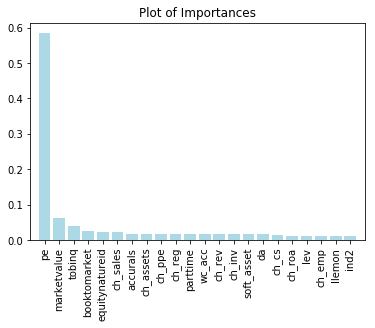
\includegraphics[width=7cm]{Tree_importance.png}  
    \end{minipage}
    }
    \subfigure[Random Forest]{
    \begin{minipage} {6cm}
    \centering
    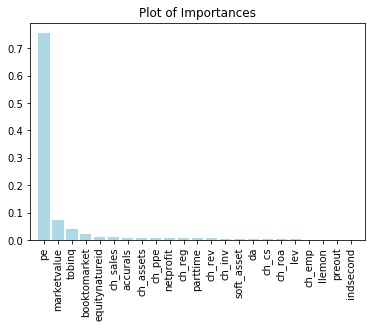
\includegraphics[width=7cm]{RF_importance.png}
    \end{minipage}
    }
    \caption{重要性排序}
\end{figure}

\subsubsection{精准度(Accuracy)}
\par 模型的精准度的是分类正确的个体再测试集中的比重。从表\ref{tab:accauc}中可以看出,logit模型的预测精准度最低只有67.3\% \footnote{若使用原始的样本,那么logit模型精准度将会只有45.3\%},这与Dechow\cite{Dechow2006The}的结果比较接近。CART算法的精准度是82.1\%。再经过最大深度选择后,决策树的精度达到84.7\%。这一结果超过了未调参的随机森林模型。后者经过调参后模型精度达到85.5\%。从精度这个角度,随机森林模型具有更好的预测力。
\subsubsection{查准率(Precision)、查全率(Recall)和F1}
模型的预测结果可以用混淆矩阵\ref{tab:confusion}表示。查准率的定义式$P(Precision) = \frac{TP}{TP+FP}$,即测试集中预测为错报的公司中真正错报的比例;查准率的定义式$R(Recall) = \frac{TP}{TP+FN}$,即测试集中所有错报的公司中被模型发现的比例;$F1$是$P$与$R$的调和平均数。传统的logit模型在查准率的表现上不如树一类的统计学习模型。同时,SMOTE算法的确能够提高查准率,而使用旧的样本更会使模型把预测值归为非异常类。这也说明原始的样本确实存在类不平衡的问题。logit模型的查准率为13\%,远低于CART和随机森林超过一半的查准率。实践中,如果利益相关者关心“错杀”的比例,那么他会更关注从查准率、查全率和F1的角度,随机森林算法具有更好的性能。

% Table generated by Excel2LaTeX from sheet 'AfterTune'
\begin{table}[H] \centering
\caption{查全率、 查准率和F1}
    \begin{tabular}{lrrr} \hline\hline
    Model & \multicolumn{1}{l}{precision} & \multicolumn{1}{l}{recall} & \multicolumn{1}{l}{F1-score} \\ \hline
    Logit & 0.132 & 0.871 & 0.229 \\
    Logit without SMOTE & 0.121 & 0.845 & 0.212 \\
    CART  & 0.500 & 0.438 & 0.467 \\
    CART without SMOTE & 0.368 & 0.541 & 0.438 \\
    Random Forest & 0.545 & 0.477 & 0.509 \\
    Random Forest without SMOTE & 0.349 & 0.574 & 0.434 \\ \hline\hline
    \end{tabular}%
  \label{tab:PrecisionRecal}%
\end{table}%

\subsection{模型的评估与调参}
\subsubsection{决策树的Max Depth}
\par 在表\ref{tab:Validation Curve for Trees}中,本文展示了利用validation curve计算不同深度训练集和测试集交叉验证得分。如果不限制最大深度,就会发生过拟合的问题,即模型在训练集与测试集上的表现发生背离。对于中国资本市场侦测财报错报的问题,本文的结果是将决策树的深度参数限制为8为最优。
\begin{figure}[htbp]
    \centering
    \subfigure[Validation Curve for Trees]{
    \begin{minipage}{6 cm}
    \centering
    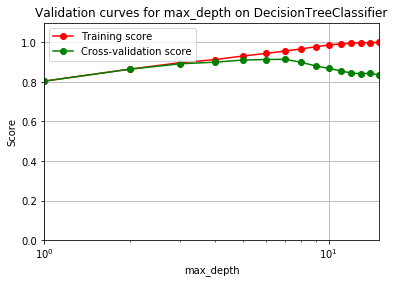
\includegraphics[width=6cm]{CART_Tune.png}
    \end{minipage}
    \label{tab:Validation Curve for Trees}
    }
    \subfigure[ROC Curve for Trees]{
    \begin{minipage} {6 cm}
    \centering
    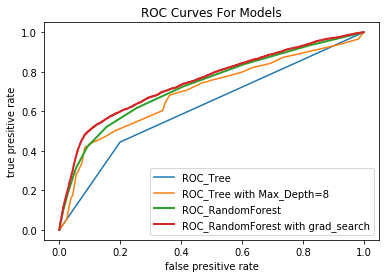
\includegraphics[width=6cm]{ROC.png}
    \end{minipage}
    \label{tab:ROC Curves}
    }
    \caption{模型评估}
\end{figure}
\subsubsection{AUC与ROC曲线}
\par 评价分类器的一个主要指标是ROC曲线和AUC值。受试者工作特征曲线 (Receiver Operating Characteristic Curve,简称ROC曲线),又称为感受性曲线(Sensitivity Curve)。最早是由Lusted\cite{Goodenough1974Radiographic}在1988年提出的。ROC曲线是以假阳性概率(False Positive Rate)为横轴,真阳性(True Positive Rate)为纵轴所组成的坐标图,和受试者在特定条件下由于采用不同的thresholds得出的不同结果画出的曲线。AUC(Area Under Curve)被定义为ROC曲线下的面积,AUC值是一个概率值\cite{Fawcett2006ROC},即当随机挑选一个正样本以及一个负样本,当前的分类算法根据计算得到的Score值将这个正样本排在负样本前面的概率。AUC值越大,当前的分类算法越有可能将正样本排在负样本前面,即能够更好的分类。
\par 本文计算了三种模型基于不同设定下的AUC\footnote{Fawcett(2006)原文:The AUC value is equivalent to the probability that a randomly chosen positive example is ranked higher than a randomly chosen negative example.}值。Logit模型的AUC值最低。决策树和随机森林的结果比较接近,均超过了0.7。同时,这一结果略弱于David和Hansen等人\cite{} 利用Rule Ensemble得到的AUC。据此,本文认为对于财务报表错报侦测的问题,决策树分类器比logit模型根据有预测能力,能够辅助利益相关者进行决策。
% Table generated by Excel2LaTeX from sheet 'AfterTune'
\begin{table}[htbp]
  \centering
  \caption{精准度与AUC}
    \begin{tabular}{llll} \hline\hline
    Model & Accuracy & AUC   & std \\ \hline
    Logit & \multicolumn{1}{r}{0.673} & \multicolumn{1}{r}{0.595} & \multicolumn{1}{r}{0.016} \\
    CART  & \multicolumn{1}{r}{0.821} & \multicolumn{1}{r}{0.693} & \multicolumn{1}{r}{0.026} \\
    Tree with max\_depth = 8 & \multicolumn{1}{r}{0.847} & \multicolumn{1}{r}{0.539} & \multicolumn{1}{r}{0.016} \\
    Random Forest & \multicolumn{1}{r}{0.832} & \multicolumn{1}{r}{0.736} & \multicolumn{1}{r}{0.009} \\
    Random Forest with tunning & \multicolumn{1}{r}{0.855} & \multicolumn{1}{r}{0.763} & \multicolumn{1}{r}{0.007} \\ \hline
    \multicolumn{4}{l}{Note: SMOTE is used before modeling} \\ \hline\hline
    \end{tabular}%
  \label{tab:accauc}%
\end{table}%
\subsubsection{随机森林调参}
\label{par:梯度优化调参}
本文进一步对随机森林模型使用梯度优化模型进行调参。在python中可以直接调用gridsearch进行并行调参。调整的参数包括:1) 混乱都下降标准选择“基尼系数”还是“信息熵”;2) 最大深度;3) 单个模型最大特征数目;4) 迭代次数。具体操作见代码源。调参的结果为一个最大深度为12、特征数位5、迭代次数为31的使用'Entropy'为标准的模型。调参使得随机森林模型预测能力提升:模型精确度上升85.5\%,模型AUC达到0.763。
% paragraph  (end)

\section{结论与反思}
\par 本文基于2002年至2017年中国资本市场的数据,通过三个统计学习模型来预测上市公司财务报表错报。在进行预测前,本文首先对原始样本使用SMOTE算法进行过采样,以处理原始样本中类不平衡的问题。之后本文使用python编写了一个进行预测的类,并进行logit模型、CART和随机森林的算法的预测与评估。研究结果显示:类不平衡的问题确实存在与财务报表错报的预测问题之中,而SMOTE算法确实能够提升三个模型查准率;传统的logit模型在中国资本市场进行预测的精准度为67.3\%,而决策树类的模型精准度有80\%以上而且具有更大的AUC值。这些结论告诉足以说明,本文的框架下,决策树类的统计学习模型对于财务报表的错报更具有预测力、性能更好。最后,本文使用梯度优化法来实现对于随机森林模型的自动调参,调参后的模型性能更佳。
\par 本文意义是为利益相关这判别某公司是否具有财务报表错报提供只管的决策辅助。在实际使用中,利益相关者如对冲基金研究员会更多的在意某一家或者某一个具体行业的上市公司是否发生重大错报,而不是概率平均值。统计学习的模型提供了一个近乎于黑箱的解决思路,可能这样的思路会在实际应用中更直观。
\par 此外,本文通过决策树类的模型得到了一个关于预测中国资本市场财报错报预测的重要性排序。在研究某一个公司是否发生财务报表错报时,优先关注重要性高的特征能够帮助利益相关方更好的了解公司的报表是否造假,并为后续的研究提供一些信息。这些特征是否有效,还有赖于更多的研究中国资本市场财报错报的文章出现。
\par 对于经济学模型来讲,统计学习的很多操作都看似“黑箱”一般,即只关注输入输出。这种模型与传统的结构方程和离散选择模型孰优孰劣不能一概而论。在过去,过度而随意的加变量,会被经济学家成为Data Mining。统计学家也将统计学习看作一种下下策的出路。然而,统计学习确实可以帮助经济学家进行变量筛选(LASSO、岭回归),为经济学研究体重很多思路。统计学习中的抽样算法能帮助解决样本的很多问题。交叉验证的思路为模型的稳健性提供支持。目前统计学习(机器学习)正在谷歌等公司的带领下,触及因果推断。
\par 本文有很多粗糙和不够完善的部分。首当其冲的是关于Y变量粗糙的选择。本文将所有的错报一视同仁,然而错报也是分危害程度的。若是将错报分成低级、中级、重大来进行学习,可能更具有实际意义。此外,本文将面板数据当作截面数据来使用,将不同年份的同一个体视作不同的个体,没有讲年份因素考虑进入上市公司特征。这样做简便,但是会损失预测力。还有一些做的不细致的地方,由于时间和精力没有做进一步探讨。

\bibliographystyle{plain}
\bibliography{termpaper}
%========================================================================
\section{附录}
\subsection{修正的Jones模型的计算} % (fold)
\label{sub:修正的Jones模型的计算}
\par 修正的jones模型在回归的过程中应当使用分行业分年份回归,其回归模型设定如下如下:
\begin{equation}
    TA_{i,t} = \beta_1(\frac{1}{A+{i,t-1}}) + \beta_2(\Delta_{i,t}-\Delta_{i,t}+\beta_3 PPE_{i,t}+\varepsilon_{i,t})
\end{equation}
\begin{equation}
    TA_{i,t} = (\Delta CRA_{i,t}-\Delta CASH_{i,t})-(\Delta CRL_{i,t}-\Delta SB_{i,t}) -\Delta DIS_{i,t}
\end{equation}
\par 其中,TA表示总应计项;$\Delta $ REV为两期营业收入的差额,:$\Delta $ REC为两期应收账款的差额;PPE是当期期末固定资产净值;A是期末资产总额;$\Delta $ CRA为当期流动资产与上期流动资产的差额;$\Delta $ CASH为当期库存现金与上期的库存现金的差额;$\Delta $ CRL为当期流动负债与上期流动负债的差额;$\Delta $ SB是当期短期借款与上期短期借款的差额;DIS是当期折旧数额。在计算TA、$\Delta $ REC、$\Delta $ REV、PPE都需要以上期期末资产进行标准化 。随后,分行业对TA进行OLS回归,所得的残差为操控性应计利润 (DA)

% subsection  (end)

\subsection{描述性统计表2} % (fold)
\label{sub:描述性统计表2} 
\par 这是好公司和坏公司的描述性统计表。
% Table generated by Excel2LaTeX from sheet 'Xsum'
\begin{table}[H]
  \centering
  \caption{描述性统计表2}
    \begin{tabular}{lrrrr} \hline\hline
          & \multicolumn{2}{c}{lemon = 1} & \multicolumn{2}{c}{lemon=0} \\
    \cmidrule{2-5}    Variable & \multicolumn{1}{l}{Obs} & \multicolumn{1}{l}{Mean} & \multicolumn{1}{l}{Obs} & \multicolumn{1}{l}{Mean} \\
    ch\_sales & 5,044 & 3.755355 & 25,720 & -8.32032 \\
    ch\_assets & 4,949 & 1.352118 & 24,922 & 0.584309 \\
    ch\_ppe & 4,944 & 9.302766 & 24,904 & 63.73016 \\
    ch\_reg & 5,112 & 1.390063 & 26,764 & 1.416866 \\
    wc\_acc & 4,031 & -0.0031 & 21,154 & 0.001648 \\
    ch\_rev & 4,708 & 0.009332 & 23,904 & 0.012919 \\
    soft\_asset & 5,112 & 0.764053 & 26,764 & 0.754902 \\
    da    & 4,629 & -2.44E+08 & 23,402 & -3.26E+08 \\
    ch\_cs & 4,676 & 2.52E+09 & 23,645 & 6.61E+09 \\
    ch\_roa & 4,738 & 0.000656 & 23,951 & 0.006194 \\
    lev   & 5,112 & 0.56417 & 26,764 & 0.524005 \\
    ch\_emp & 4,723 & 1.130992 & 23,954 & 1.05698 \\
    llemon & 4,742 & 0.540489 & 24,043 & 0.093666 \\
    marketvalue & 5,112 & 8.22E+09 & 26,764 & 1.45E+10 \\
    tobinq & 5,112 & 2.819399 & 26,764 & 4.33967 \\
    booktomarket & 5,112 & 0.993255 & 26,764 & 1.051638 \\ \hline\hline
    \end{tabular}%
  \label{tab:描述性统计表2}%
\end{table}%

% subsection 描述性统计表2 (end)


\subsection{SMOTE的伪代码} % (fold)
\label{sub:smote的伪代码}
这是从Chawla\cite{Chawla2002SMOTE}原文中抄录的算法:
\scriptsize
\begin{lstlisting}
Algorithm SMOTE(T, N, k)
Input: Number of minority class samples T; Amount of SMOTE N%; Number of nearest
neighbors k
Output: (N/100)* T synthetic minority class samples
1. (∗ If N is less than 100%, randomize the minority class samples as only a random
percent of them will be SMOTEd. ∗)
2. if N <100
3. then Randomize the T minority class samples
4. T = (N/100) ∗ T
5. N = 100
6. endif
7. N = (int)(N/100)( ∗ The amount of SMOTE is assumed to be in integral multiples of
100. ∗)
8. k = Number of nearest neighbors
9. numattrs = Number of attributes
10. Sample[ ][ ]: array for original minority class samples
11. newindex: keeps a count of number of synthetic samples generated, initialized to 0
12. Synthetic[ ][ ]: array for synthetic samples
(∗ Compute k nearest neighbors for each minority class sample only. ∗)
13. for i ← 1 to T
14. Compute k nearest neighbors for i, and save the indices in the nnarray
15. Populate(N, i, nnarray)
16. endfor
Populate(N, i, nnarray) (∗ Function to generate the synthetic samples. ∗)
17. while N != 0
18. Choose a random number between 1 and k, call it nn. This step chooses one of
the k nearest neighbors of i.
19. for attr ← 1 to numattrs
20. Compute: dif = Sample[nnarray[nn]][attr] − Sample[i][attr]
21. Compute: gap = random number between 0 and 1
22. Synthetic[newindex][attr] = Sample[i][attr] + gap ∗ dif
23. endfor
24. newindex++
25. N = N − 1
26. endwhile
27. return (∗ End of Populate. ∗)   
\end{lstlisting}
% subsection smote的伪代码 (end)

\subsection{随机森林和Bagging算法的思想} % (fold)
\label{sub:bagging算法的思想}
\normalsize

\par bagging的算法过程如下: 
\begin{itemize}
    \item 从原始样本集中使用Bootstraping方法随机抽取n个训练样本,共进行k轮抽取,得到k个训练集。(k个训练集之间相互独立,元素可以有重复)
    \item 对于k个训练集,我们训练k个模型(这k个模型可以根据具体问题而定,比如决策树,knn等)
    \item 对于分类问题:由投票表决产生分类结果;对于回归问题:由k个模型预测结果的均值作为最后预测结果。(所有模型的重要性相同)
\end{itemize}

\par 随机森林根据下列算法而建造每棵树: 
\begin{itemize}
    \item 用N来表示训练用例(样本)的个数,M表示特征数目。
    \item 输入特征数目m,用于确定决策树上一个节点的决策结果;其中m应远小于M。
    \item 从N个训练用例(样本)中以有放回抽样的方式,取样N次,形成一个训练集(即bootstrap取样),并用未抽到的用例(样本)作预测,评估其误差。
    \item  对于每一个节点,随机选择m个特征,决策树上每个节点的决定都是基于这些特征确定的。根据这m个特征,计算其最佳的分裂方式。
    \item 每棵树都会完整成长而不会剪枝(Pruning,这有可能在建完一棵正常树状分类器后会被采用)。
\end{itemize}

\subsection{混淆矩阵} % (fold)
\label{sub:混淆矩阵}
% Table generated by Excel2LaTeX from sheet 'AfterTune'
\begin{table}[htbp] \centering
\caption{混淆矩阵}
    \begin{tabular}{c|r|l|l}
    \hline\hline
    \multicolumn{2}{c|}{\multirow{2}[4]{*}{A Model}} & \multicolumn{2}{c}{prediction} \\
    \cmidrule{3-4}    \multicolumn{2}{c|}{} & \multicolumn{1}{r|}{0} & \multicolumn{1}{r}{1} \\
    \midrule
    \multirow{2}[4]{*}{actual } & 0     & TN    & FP \\
    \cmidrule{2-4}          & 1     & FN    & TP \\
    \hline\hline
    \end{tabular}%
  \label{tab:confusion}%
\end{table}%




\end{spacing}
\end{document}